\documentclass{ecnreport}

\stud{M2 IMARO \& OD Robotique}
\topic{Aerial and underwater robots}

\begin{document}

\inserttitle{Aerial and underwater drones}

\insertsubtitle{AUV simulation and control}

\section{Content of this lab}

The goal of this lab is to control a thruster-propelled Autonomous Underwater Vehicle (AUV). The AUV should be able to follow a trajectory defined with a sequence of waypoints, and estimate its pose from an EKF.

\subsection{The simulation}

The simulation is run through Gazebo, which handles hydrodynamics, thrusters and sensors.
The actual package that you will modify is to be cloned in \okt{\~/ros2/src} with:
\begin{bashcodelarge}
cd ~/ros2/src
git clone https://github.com/oKermorgant/ecn_auv_lab
cd ecn_auv_lab
ros2ws && colbuild -t # compile this
\end{bashcodelarge}

This package has a classical ROS structure:
\begin{figure}[h]
\begin{minipage}{.25\linewidth} ~ \end{minipage}
\begin{minipage}{.5\linewidth}
 \dirtree{%
.1 ecn\_auv\_lab.
.2 launch.
.2 params.
.2 src.
.2 urdf.
.2 package.xml.
.2 CMakeLists.txt.
}
\end{minipage}
%\begin{minipage}{.2\linewidth} ~ \end{minipage}
\caption{Files used by the simulator}
\end{figure}

QtCreator can be automatically configured by calling \okt{ideconf} from the \okt{ecn_auv_lab} package.

The simulation is run with:
\begin{bashcodelarge}
 ros2 launch ecn_auv_lab sim_launch.py
\end{bashcodelarge}

The main option is \okt{gt:=false}. This will prevent the simulator to output the ground truth and force the control to rely on sensor feedback. This will be used in the second part of the lab.

\section{Waypoint following}

The first task is to finish the waypoint following node defined in \okt{waypoint.cpp}. This node already loads the waypoints defined in \okt{waypoints.yaml} but does not follow them yet.
These waypoints should be modified according to the trajectory you want the robot to follow. A waypoint is defined by its $(x,y,z,\theta)$ values where $\theta$ is the yaw angle. Look at the current
code to see how to change a yaw angle to a quaternion needed by the \okt{PoseStamped} message.\\

Topics can be renamed or the node can be run through a launch file in order to be in the \okt{/bluerov2} namespace. The low-level control (e.g. PIDs) is run through:
\begin{bashcodelarge}
 ros2 launch ecn_auv_lab control_launch.py
 \end{bashcodelarge}

 The \okt{manual} option (default True) will show sliders to give the pose setpoint. When testing your own code, run the control launch file with \okt{manual:=false}.
This leads to the following graph where \okt{/bluerov2/waypoints} is your node.
\begin{figure}[h]\centering
 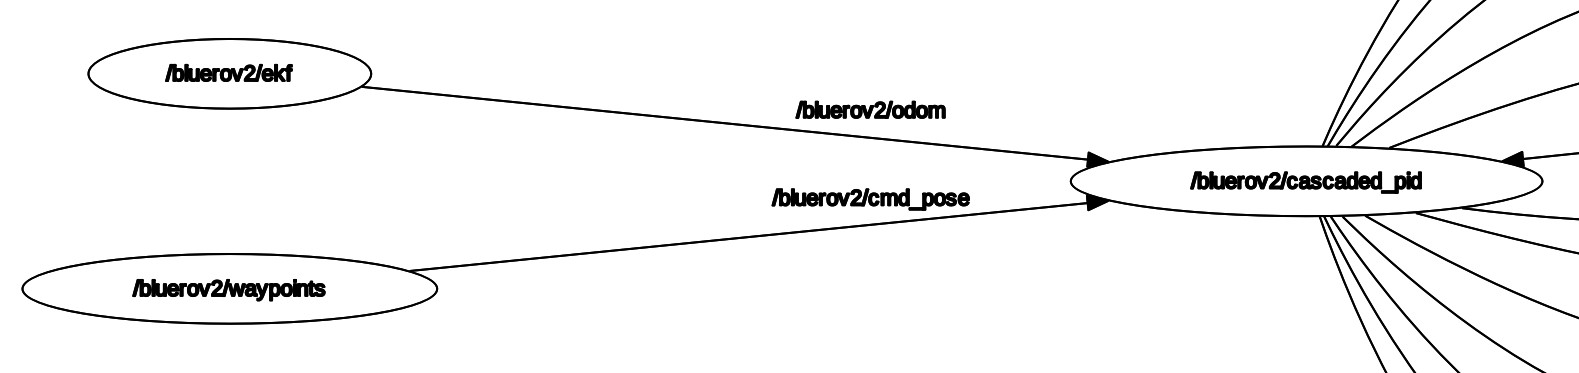
\includegraphics[width=.8\linewidth]{graph}
\end{figure}

Two GUI are launched: 
\begin{itemize}
 \item Gazebo is the simulator
 \item RViz is a visualizer and displays the current pose estimate (red) and the current waypoint to be followed (3D frame)
\end{itemize}

Manually defined setpoints can be easily published by using \okt{manual:=true} (default).\\

The goal is to modify the source and waypoint list in order to loop through the waypoints (go back to waypoint 0 after the last one was reached).
The structure of the \okt{setpoint} message can be found with:
\begin{bashcodelarge}
ros2 interface show geometry_msgs/msg/PoseStamped
\end{bashcodelarge}
which gives:
\begin{bashcodelarge}
std_msgs/Header header
  uint32 seq
  time stamp
  string frame_id
geometry_msgs/Pose pose
  geometry_msgs/Point position
    float64 x
    float64 y
    float64 z
  geometry_msgs/Quaternion orientation
    float64 x
    float64 y
    float64 z
    float64 w
\end{bashcodelarge}
The header is already written but you have to define the pose section from the reading of the loaded waypoint file.\\

Remember that the AUV may not reach perfectly the desired position, so you should cycle to the next waypoint when the position error is below a given threshold.
Two thresholds are loaded from the YAML file: \okt{position_thr} and \okt{orientation_thr}, that may be tuned accordingly to the desired accuracy.\\
The current position of the AUV can be found on the topic \okt{/bluerov2/state} and is of type \okt{nav_msgs/Odometry} with a structure similar to \okt{geometry_msgs/PoseStamped}, and where we are interested only
in the \okt{pose} section.\\

Once the waypoint node works, uncomment the corresponding line in \okt{control_launch.py} so this launch file runs it when \okt{manual:=false}.


%\section{Modification and tuning of the robot}
%
%The underwater robot itself is defined in the \okt{auv.xacro} file. Check the available sensors and thrusters and find the available motions from the thruster map.
%You can add or modify the thrusters if needed. The thruster control matrix is computed automatically, however the gains of the PID are not tuned accordingly.

%\subsection{Basics of URDF}
%
%The \okt{xacro} format allows using variables to generate the URDF model of a robot.
%In this format, the robot is composed of links and joints. In our case we will assume that the AUV has only one link and no joints.
%
%In the example the AUV is composed of one cylinder, which is described under the \okt{visual} tag.
%A tutorial is available at \okt{http://wiki.ros.org/urdf/Tutorials/Building a Visual Robot Model with URDF from Scratch}
%
%In addition to the main body, thruster links can be defined with the \okt{xacro:thruster_link} tag, as  shown in the example.
%The xyz position and the roll-pitch-yaw orientation between the main body and the thruster has to be indicated.

%\section{Low-level tuning}
%
%The gains of the PID can be tuned online through Dynamic Reconfigure in (\okt{rqt}).
%The Dynamic Reconfigure plugin can be used to change the PID gains without exiting the simulator.
%Once acceptable values have been found for the gains, you may update the \okt{auv_control.yaml} file to set the default values.

\section{Pose estimation from Extended Kalman Filter}

The architecture used until then is quite unrealistic.
Indeed, data on the topic \okt{/bluerov2/pose} is the ground truth in terms of absolute position and velocity of the AUV (it is coming
directly from the simulator).
In this section we will replace it by an EKF estimator and see the problems that arise.

Here, Gazebo is still publishing the ground truth but on the \okt{/bluerov2/pose_gt} topic. This data is processed (noise is added) and republished from two simulated sensors:
\begin{enumerate}
  \item A depth sensor publishing a pose on \okt{/bluerov2/depth} where only the Z-position is meaningful
  \item A USBL device publishing a pose on \okt{/bluerov2/usbl} where only the (X,Y,Z) positions are meaningful
\end{enumerate}
Gazebo is also publishing simulated IMU data on the \okt{/bluerov2/lsm} and \okt{/bluerov2/mpu} topics.
Finally, RViz displays the estimate of the AUV (in red).
For comparison purpose, the ground truth is displayed in blue. The setpoint is still displayed as a 3D frame.

The sensor data (depth, USBL and 2 IMU) should be fused by the EKF node in order to output an estimate of the state on the \okt{/bluerov2/odom} and \okt{/tf} topics that are used by the PID and your waypoint node.

The previous launch files should be run as:
\begin{bashcodelarge}
# run the simulation without ground truth
ros2 launch ecn_auv_lab sim_launch.py gt:=false
# run the control and track waypoints
ros2 launch ecn_auv_lab control_launch.py manual:=false
 \end{bashcodelarge}

Then the EKF can be run with:
 \begin{bashcodelarge}
ros2 launch ecn_auv_lab ekf_launch.py
 \end{bashcodelarge}

The parameter file of the EKF is at \okt{params/ekf.yaml}. It relies on the \link{http://docs.ros.org/en/noetic/api/robot_localization/html/index.html}{\okt{robot_localization}} package, which offers generic EKF in SE(3). This node creates a 15-components (6 pose, 6 velocities and 3 accelerations) state estimate.\\

The EKF node can accept any number of input measurements, written as parameters:
\begin{itemize}
 \item \okt{odom#} for odometry
 \item \okt{imu#}  for imu
 \item \okt{pose#} for pose
\end{itemize}
Then the corresponding \okt{<param>_config} parameter is a list of 15 Boolean's indicating which part of the state is to be obtained with this topic. \\

The parameter file should be modified so that the EKF node
subscribes to the available data topics. The Boolean tables should
also be updated in order to tell which components of the state are measured by each of the sensors.

You can see the impact of each sensor by running the EKF with:
\begin{enumerate}
 \item only one or two IMU's
 \item IMU's and depth sensor
 \item All sensors (IMU, depth, usbl)
\end{enumerate}

You can also change the \okt{params/noise.yaml} file to increase the noise of the simulated sensors and see the consequences in the EKF






\end{document}
